\chapter{Solving for Camera Poses Based on Images}
\label{ch:sfm}

The ASP tool \texttt{camera\_solve} offers several ways
to find the true position of frame camera images that do
not come with any attached pose metadata. This can be useful with
aerial, hand-held, and historical imagery for which such information
may be incomplete or inaccurate.

An overview of the tool and examples are provided in this chapter.
Reference information for this tool can be found in Appendix
\ref{camerasolve}.

This tool can be optionally bypassed if, for example, the longitude and latitude of
the corners of all images are known (section \ref{imagecorners}). 

\section{Camera Solve Overview}

The \texttt{camera\_solve} tool is implemented as a Python wrapper around
two other tools.  The first of these is the the THEIA software library,
which is used to generate initial camera position estimates in a local
coordinate space.  You can learn more about THEIA at
\url{http://www.theia-sfm.org/index.html}.  The second tool is ASP's
own \texttt{bundle\_adjust} tool.  The second step improves the solution
to account for lens distortion and transforms the solution from local
to global coordinates by making use of additional input data.

The tool only solves for the extrinsic camera parameters
and the user must provide intrinsic camera information.
You can use the \texttt{camera\_calibrate}
tool (see Appendix \ref{cameracalibrate}) or other camera calibration software
to solve for intrinsic parameters if you have access to the camera in question.
The camera calibration information must be contained in a
.tsai pinhole camera model file and must passed in using the
\texttt{-\/-calib-file} option.  You can find descriptions of
our supported pinhole camera models in Appendix \ref{chapter:pinholemodels}.

If no intrinsic camera information is known, it can be guessed by doing some experimentation.
This is discussed in section \ref{findintrinsics}.

In order to transform the camera models from local to world coordinates,
one of three pieces of information may be used.  These sources are listed
below and described in more detail in the examples that follow:
\begin{itemize}{}
\item A set of ground control points of the same type used by \texttt{pc\_align}.
The easiest way to generate these points is to use the ground control point
writer tool available in the \texttt{stereo-gui} tool.
\item A set of estimated camera positions (perhaps from a GPS unit) stored in
a csv file.
\item A DEM which a local point cloud can be registered to using \texttt{pc\_align}.
This method can be more accurate if estimated camera positions are also used.  The user
must perform alignment to a DEM, that step is not handled by \texttt{camera\_solve}.
\end{itemize}{}

Power users can tweak the individual steps that \texttt{camera\_solve} goes through
to optimize their results.  This primarily involves setting up a custom flag file for
THEIA and/or passing in settings to \texttt{bundle\_adjust}.

\section{Example: Apollo 15 Metric Camera}
\label{sfm:generic}

To demonstrate the ability of the Ames Stereo Pipeline to process a
generic frame camera we use images from the Apollo 15 Metric camera.  The
 calibration information for this camera is available online and we have accurate
 digital terrain models we can use to verify our results.

First download a pair of images:

\begin{verbatim}
> wget http://apollo.sese.asu.edu/data/metric/AS15/png/AS15-M-0414_MED.png
> wget http://apollo.sese.asu.edu/data/metric/AS15/png/AS15-M-1134_MED.png
\end{verbatim}

\begin{figure}[h!]
\centering
  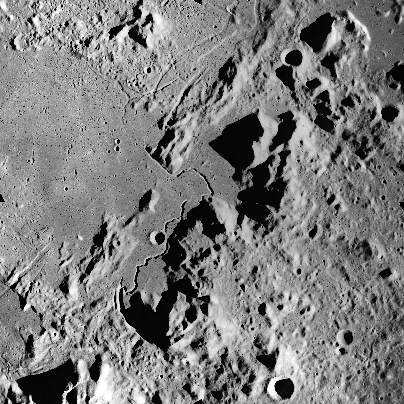
\includegraphics[width=3.0in]{images/examples/pinhole/AS15-M-0414.png}
  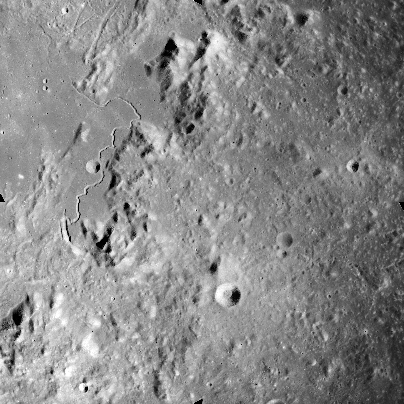
\includegraphics[width=3.0in]{images/examples/pinhole/AS15-M-1134.png}
\caption{The two Apollo 15 images.}
\label{fig:pinhole-a15-input-images}
\end{figure}

In order to make the example run faster we use downsampled versions of
the original images.  The images at those links have already been downsampled
by a factor of 4*sqrt(2) from the original images.  This means that the
effective pixel size has increased from five microns (0.005 millimeters) to
0.028284 millimeters.

The next step is to fill out the rest of the pinhole camera model information
we need.  Using the data sheets available at 
\url{http://apollo.sese.asu.edu/SUPPORT_DATA/AS15_SIMBAY_SUMMARY.pdf} 
we can find the lens distortion parameters for metric camera.  Looking at the 
ASP lens distortion models in Appendix \ref{chapter:pinholemodels}, 
we see that the description matches ASP's Brown-Conrady model.  
Using the example in the appendix we can fill out
the rest of the sensor model file (metric\_model.tsai) so it looks as follows:

\begin{verbatim}
VERSION_3
fu = 76.080
fv = 76.080
cu = 57.246816
cv = 57.246816
u_direction = 1  0  0
v_direction = 0  1  0
w_direction = 0  0  1
C = 0 0 0
R = 1 0 0 0 1 0 0 0 1
pitch = 0.028284
BrownConrady
xp = -0.006
yp = -0.002
k1 = -0.13361854e-5
k2 = 0.52261757e-09
k3 = -0.50728336e-13
p1 = -0.54958195e-06
p2 = -0.46089420e-10
phi = 2.9659070
\end{verbatim}

These parameters use units of millimeters so we have to convert the nominal center
point of the images from 2024 pixels to units of millimeters.  Note that for some older
images like these the nominal image center can be checked by looking for some sort of
marking around the image borders that indicates where the center should lie.  For these
pictures there are black triangles at the center positions and they line up nicely
with the center of the image.  Before we try to solve for the camera positions we can run
a simple tool to check the quality of our camera model file:
\begin{verbatim}
> undistort_image AS15-M-0414_MED.png metric_model.tsai -o corrected_414.tif
\end{verbatim}

It is difficult to tell if the distortion model is correct by using this
tool but it should be obvious if there are any gross errors in your
camera model file such as incorrect units or missing parameters.  In this
case the tool will fail to run or will produce a significantly distorted image.
For certain distortion models the \texttt{undistort\_image} tool may take a long time to run.

If your input images are not all from the same camera or were scanned such that the center
point is not at the same pixel, you can run \texttt{camera\_solve} with one camera
model file per input image.  To do so pass a space-separated list of files 
surrounded by quotes to the \texttt{--calib-file} option such as 
\texttt{--calib-file "c1.tsai c2.tsai c3.tsai"}.

If we do not see any obvious problems we can go ahead and run the \texttt{camera\_solve} tool:
\begin{verbatim}
> camera_solve out/ AS15-M-0414_MED.png AS15-M-1134_MED.png --datum D_MOON \
  --calib-file metric_model.tsai
\end{verbatim}

We should get some camera models in the output folder and see a printout of
the final bundle adjustment error among the program output information:
\begin{verbatim}
Cost:
Initial                          1.450385e+01
Final                            7.461198e+00
Change                           7.042649e+00
\end{verbatim}

We can't generate a DEM with these local camera models but we can run stereo anyways
and look at the intersection error in the fourth band of the \texttt{PC.tif} file.  While
there are many speckles in this example where stereo correlation failed the mean
intersection error is low and we don't see any evidence of lens distortion error.

\begin{verbatim}
> stereo AS15-M-0414_MED.png AS15-M-1134_MED.png out/AS15-M-0414_MED.png.final.tsai \
  out/AS15-M-1134_MED.png.final.tsai -t pinhole s_local/out  --corr-timeout 300 \
  --erode-max-size 100
> gdalinfo -stats s_local/out-PC.tif
...
Band 4 Block=256x256 Type=Float32, ColorInterp=Undefined
  Minimum=0.000, Maximum=56.845, Mean=0.340, StdDev=3.512
  Metadata:
    STATISTICS_MAXIMUM=56.844654083252
    STATISTICS_MEAN=0.33962282293374
    STATISTICS_MINIMUM=0
    STATISTICS_STDDEV=3.5124044818554
\end{verbatim}

The tool \texttt{point2mesh} (section \ref{point2mesh}) can be used to
obtain a visualizable mesh from the point cloud. 

In order to generate a useful DEM, we need to move our cameras from local coordinates
to global coordinates.  The easiest way to do this is to obtain known ground control
points (GCPs) which can be identified in the frame images.  This will allow an accurate
positioning of the cameras provided that the GCPs and the camera model parameters are
accurate.  To create GCPs see the instructions for the \texttt{stereo\_gui} tool in
appendix \ref{bagcp}.
For the Moon there are several ways to get DEMs and in this case we generated GCPs
using \texttt{stereo\_gui} and a DEM generated from LRONAC images.

After running this command:
\begin{verbatim}
> camera_solve out_gcp/ AS15-M-0414_MED.png AS15-M-1134_MED.png --datum D_MOON \
  --calib-file metric_model.tsai --gcp-file ground_control_points.gcp
\end{verbatim}
we end up with results that can be compared with the a DEM created from LRONAC images.
The stereo results on the Apollo 15 images leave something to be desired but the
DEM they produced has been moved to the correct location.  You can easily visualize
the output camera positions using the \texttt{orbitviz} tool with the
\texttt{--load-camera-solve} option as shown below.  Green lines between camera
positions mean that a sufficient number of matching interest points were found
between those two images.

\begin{verbatim}
> stereo AS15-M-0414_MED.png AS15-M-1134_MED.png out_gcp/AS15-M-0414_MED.png.final.tsai \
  out_gcp/AS15-M-1134_MED.png.final.tsai -t nadirpinhole s_global/out  --corr-timeout 300 \
  --erode-max-size 100
> orbitviz -t nadirpinhole -r moon out_gcp --load-camera-solve
\end{verbatim}


\begin{figure}[h!]
\centering
  \subfigure[{\tt orbitviz display}]{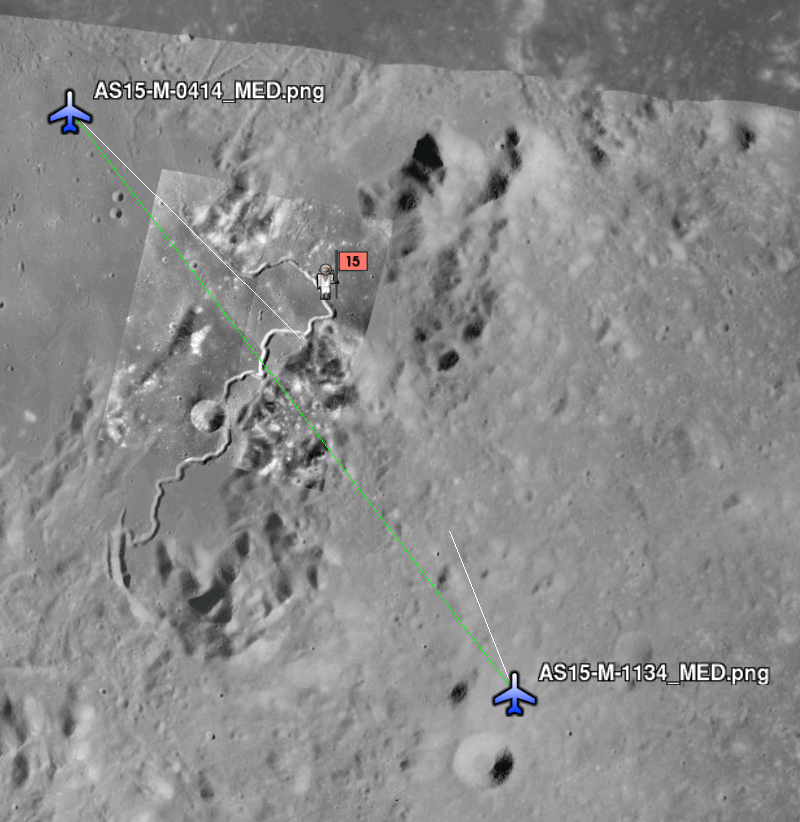
\includegraphics[width=3.5in]{images/examples/pinhole/a15_orbitviz_display.png}}
  \hfil
  \subfigure[{\tt KML Screenshot}]{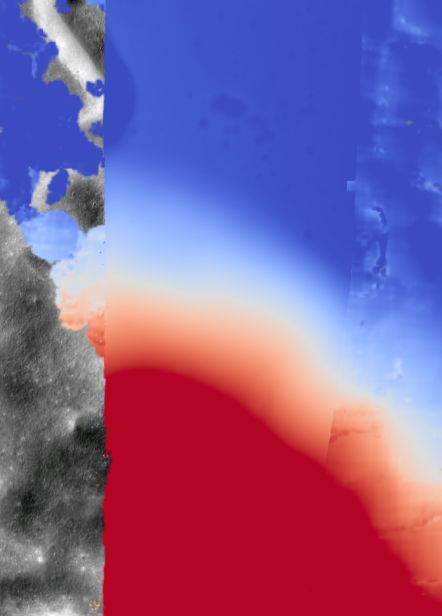
\includegraphics[width=3in]{images/examples/pinhole/a15_image_diff.png}}
\caption{(a) Solved for camera positions plotted using orbitviz.  (b) A narrow LRONAC DEM overlaid on the resulting DEM, both colormapped to the same elevation range.}
\label{fig:pinhole-a15-result-image}
\end{figure}

ASP also supports the method of initializing the \texttt{camera\_solve} tool with estimated
camera positions.  This method will not move the cameras to exactly the right location but
it should get them fairly close and at the correct scale, hopefully close enough
to be used as-is or to be refined using \texttt{pc\_align} or some other method.
To use this method, pass additional bundle adjust parameters to \texttt{camera\_solve} similar to the following line:

\begin{verbatim}
--bundle-adjust-params '--camera-positions nav.csv \
 --csv-format "1:file 12:lat 13:lon 14:height_above_datum" --camera-weight 0.2'
\end{verbatim}

The nav data file you use must have a column (the "file" column) containing a string that can be matched to the
input image files passed to \texttt{camera\_solve}.  The tool looks for strings that are fully contained
inside one of the image file names, so for example the field value \texttt{2009\_10\_20\_0778} would be
matched with the input file \texttt{2009\_10\_20\_0778.JPG}.

Chapter \ref{nextsteps} will discuss the \texttt{stereo} program in more
detail and the other tools in ASP.

\section{Example: IceBridge DMS Camera}
\label{sfm:icebridge}


The DMS (Digital Mapping System) Camera is a frame camera flown on as part of the NASA
IceBridge program to collect digital terrain imagery of polar and Antarctic terrain
(\url{http://nsidc.org/icebridge/portal/}). 

To process this data the steps are very similar to the steps described
above for the Apollo Metric camera but there are some aspects which are
particular to IceBridge.  You can download DMS images from
\url{ftp://n5eil01u.ecs.nsidc.org/SAN2/ICEBRIDGE_FTP/IODMS0_DMSraw_v01/}.
A list of the available data types can be found at
\url{https://nsidc.org/data/icebridge/instr_data_summary.html}.  This
example uses data from the November 5, 2009 flight over Antarctica. The
following camera model (icebridge\_model.tsai) was used (see chapter
\ref{chapter:pinholemodels} on camera models):

\begin{verbatim}
VERSION_3
fu = 28.429
fv = 28.429
cu = 17.9712
cv = 11.9808
u_direction = 1  0  0
v_direction = 0  1  0
w_direction = 0  0  1
C = 0 0 0
R = 1 0 0 0 1 0 0 0 1
pitch = 0.0064
Photometrix
xp = 0.004
yp = -0.191
k1 = 1.31024e-04
k2 = -2.05354e-07
k3 = -5.28558e-011
p1 = 7.2359e-006
p2 = 2.2656e-006
b1 = 0.0
b2 = 0.0
\end{verbatim}

Note that these images are RGB format which is not supported by all ASP tools.  
To use the files with ASP, first convert them to single channel images using 
a tool such as ImageMagick's \texttt{convert}, \texttt{gdal\_translate}, or 
\texttt{gdal\_edit.py}. Different conversion methods may produce slightly different
results depending on the contents of your input images.
Some conversion command examples are shown below:

\begin{verbatim}
convert rgb.jpg -colorspace Gray gray.jpg
gdal_calc.py  --overwrite --type=Float32 --NoDataValue=-32768       \
  -A rgb.tif --A_band=1 -B rgb.tif --B_band=2 -C rgb.tif            \
  --C_band=3 --outfile=gray.tif --calc="A*0.2989+B*0.5870+C*0.1140"
gdal_translate -b 1 rgb.jpg gray.jpg
\end{verbatim}

In the third command we used \texttt{gdal\_translate} to pick a single
band rather than combining the three.

Obtaining ground control points for icy locations on Earth can be particularly difficult because
they are not well surveyed or because the terrain shifts over time.
This may force you to use estimated camera positions
to convert the local camera models into global coordinates.
To make this easier for IceBridge data sets, ASP provides the
\texttt{icebridge\_kmz\_to\_csv} tool (see appendix \ref{icebridgekmztocsv})
which extracts a list of estimated camera positions from the kmz files available for each
IceBridge flight at \url{http://asapdata.arc.nasa.gov/dms/missions.html}.

Another option which is useful when processing IceBridge data is the
\texttt{-\/-position-filter-dist} option for \texttt{bundle\_adjust}.  IceBridge data sets contain
a large number of images and when processing many at once you can significantly decrease
your processing time by using this option to limit interest-point matching to image pairs
which are actually close enough to overlap.  A good way to determine what distance to use
is to load the camera position kmz file from their website into Google Earth and use the
ruler tool to measure the distance between a pair of frames that are as far apart as you
want to match. Commands using these options may look like this:

\begin{verbatim}
icebridge_kmz_to_csv  1000123_DMS_Frame_Events.kmz  camera_positions.csv
camera_solve out 2009_11_05_00667.JPG 2009_11_05_00668.JPG  \
  2009_11_05_00669.JPG 2009_11_05_00670.JPG  2009_11_05_02947.JPG 2009_11_05_02948.JPG \
  2009_11_05_02949.JPG  2009_11_05_02950.JPG  2009_11_05_01381.JPG 2009_11_05_01382.JPG  \
  --datum WGS84 --calib-file icebridge_model.tsai  \
  --bundle-adjust-params '--camera-positions camera_positions.csv \
  --csv-format "1:file 2:lon 3:lat 4:height_above_datum" --position-filter-dist 2000'
orbitviz out --load-camera-solve --hide-labels -r wgs84 -t nadirpinhole
\end{verbatim}

Alternatively, the \texttt{camera\_solve} executable can be bypassed
altogether.  If a given image has already an orthoimage associated with
it (check the IceBridge portal page), that provides enough information
to guess an initial position of the camera, using the
\texttt{ortho2pinhole} tool. Later, the obtained cameras can be
bundle-adjusted. Here is how this tool can be used, on grayscale images:

\begin{verbatim}
 ortho2pinhole raw_image.tif ortho_image.tif icebridge_model.tsai output_pinhole.tsai
\end{verbatim}

\begin{figure}[h!]
\centering
  \subfigure[]{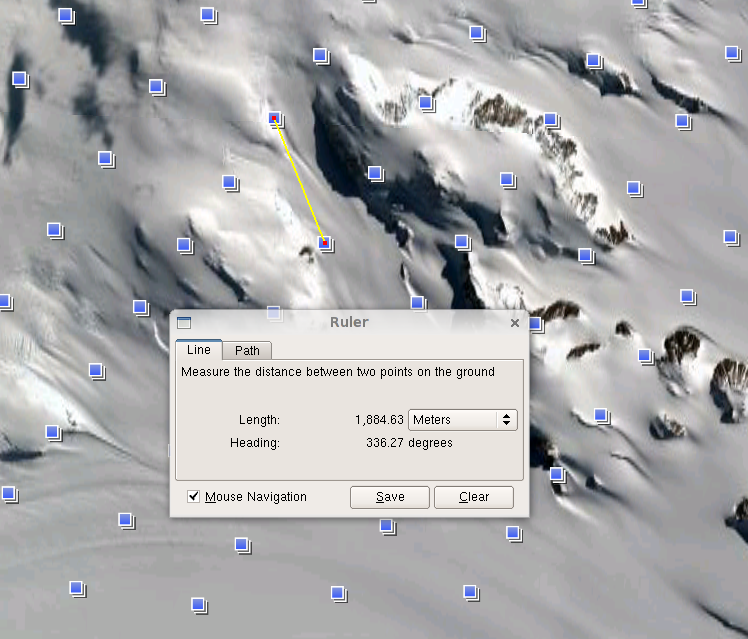
\includegraphics[width=3.5in]{images/examples/pinhole/icebridge_frame_dists.png}}
  \hfil
  \subfigure[]{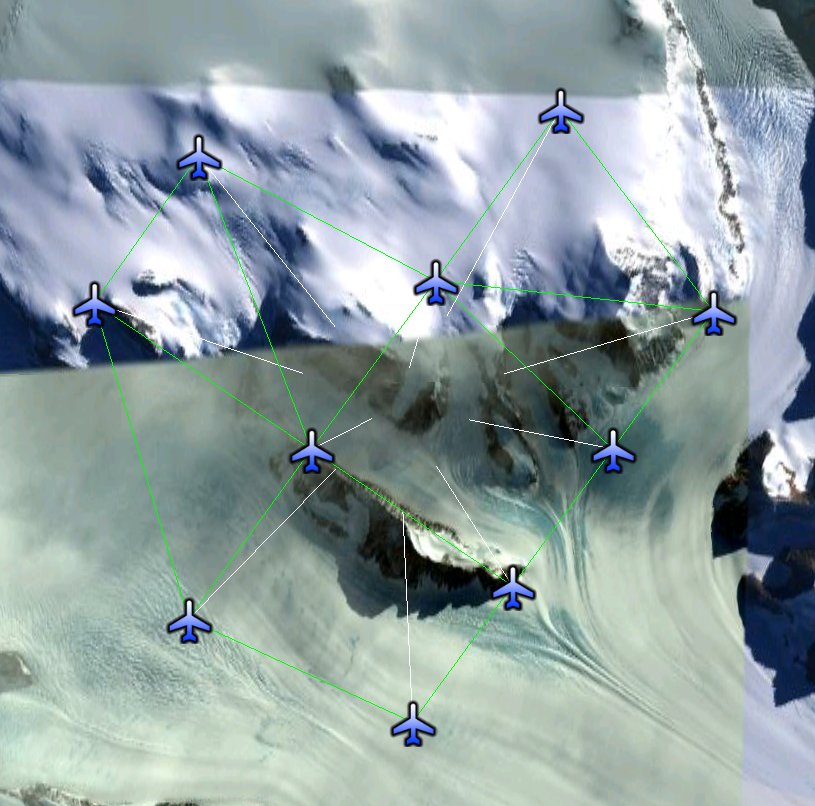
\includegraphics[width=3in]{images/examples/pinhole/icebridge_orbitviz_display.png}}
\caption{(a) Measuring the distance between estimated frame locations using Google Earth
and an IceBridge kmz file.  The kmz file is from the IceBridge website with no modifications.
Using a position filter distance of 2000 meters will mostly limit image IP matching
in this case to each image's immediate "neighbors".  (b) Display of \texttt{camera\_solve}
results for ten IceBridge images using \texttt{orbitviz}.}
\label{fig:pinhole-icebridge-camera-results}
\end{figure}


Some IceBridge flights contain data from the Land, Vegetation, and Ice Sensor (LVIS)
lidar which can be used to register DEMs created using DMS
imagery.  LVIS data can be downloaded at
\url{ftp://n5eil01u.ecs.nsidc.org/SAN2/ICEBRIDGE/ILVIS2.001/}. The lidar data comes in plain text
files that \texttt{pc\_align} and \texttt{point2dem} can parse using the following option:
\begin{verbatim}  --csv-format "5:lat 4:lon 6:height_above_datum"  \end{verbatim}
ASP provides the \texttt{lvis2kml} tool to help visualize the coverage and terrain contained
in LVIS files, see Appendix \ref{lvis2kml} for details.
The LVIS lidar coverage is sparse compared to the image coverage and you will have difficulty
getting a good registration unless the region has terrain features such as hills or you are
registering very large point clouds that overlap with the lidar coverage across a wide area.
Otherwise \texttt{pc\_align} will simply slide the flat terrain to an incorrect location to
produce a low-error fit with the narrow lidar tracks.  This test case was specifically chosen
to provide strong terrain features to make alignment more accurate but \texttt{pc\_align} still
failed to produce a good fit until the lidar point cloud was converted into a smoothed DEM.

\begin{verbatim}
stereo 2009_11_05_02948.JPG  2009_11_05_02949.JPG  out/2009_11_05_02948.JPG.final.tsai \
  out/2009_11_05_02949.JPG.final.tsai st_run/out -t nadirpinhole
point2dem ILVIS2_AQ2009_1105_R1408_055812.TXT --datum WGS_1984 \
  --t_srs "+proj=stere +lat_0=-90 +lon_0=0 +k=1 +x_0=0 +y_0=0 +datum=WGS84 +units=m +no_defs" \
  --csv-format "5:lat 4:lon 6:height_above_datum"  --tr 30  \
  --search-radius-factor 2.0 -o lvis
pc_align  --max-displacement 1000 lvis-DEM.tif st_run/out-PC.tif  -o align_run/out \
  --save-transformed-source-points --datum wgs84 --outlier-ratio 0.55
point2dem align_run/out-trans_source.tif --datum WGS_1984 \
  --t_srs "+proj=stere +lat_0=-90 +lon_0=0 +k=1 +x_0=0 +y_0=0 +datum=WGS84 +units=m +no_defs"
colormap align_run_big/out-trans_source-DEM.tif --min 200 --max 1500
colormap lvis-DEM.tif --min 200 --max 1500
image2qtree lvis-DEM_CMAP.tif
image2qtree align_run_big/out-trans_source-DEM_CMAP.tif
\end{verbatim}

\begin{figure}[h!]
\centering
  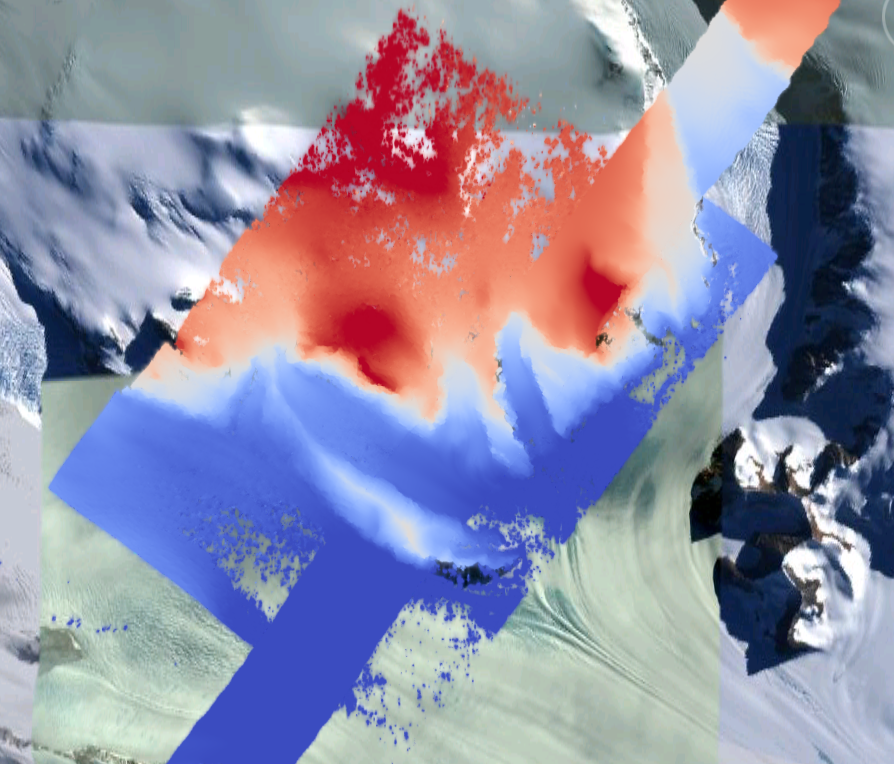
\includegraphics[width=5.5in]{images/examples/pinhole/icebridge_dem_overlay.png}
\caption{LVIS lidar DEM overlaid on the ASP created DEM, both colormapped to the same elevation range.
The ASP DEM could be improved but the registration is accurate.  Notice how narrow the LVIS lidar coverage
is compared to the field of view of the camera. You may want to experiment using the SGM algorithm to improve the coverage.}
\label{fig:pinhole-icebridge-orbitviz}
\end{figure}

Other IceBridge flights contain data from the Airborne Topographic Mapper (ATM) lidar sensor.  
Data from this sensor comes packed in one of several formats (variants of .qi or .h5) so
ASP provides the \texttt{extract\_icebridge\_ATM\_points} tool to convert them into plain
text files, which later can be read into other ASP tools using the formatting:
\begin{verbatim}
  --csv-format "1:lat 2:lon 3:height_above_datum"
\end{verbatim}
To run the tool, just pass in the name of the input file as an argument and a new file with a
csv extension will be created in the same directory.
Using the ATM sensor data is similar to using the LVIS sensor data.

For some IceBridge flights, lidar-aligned DEM files generated from the DMS
image files are available, see the web page here: \url{http://nsidc.org/data/iodms3}
These files are improperly formatted and cannot be used by ASP as is.  To correct them, run
the \texttt{correct\_icebridge\_l3\_dem} tool as follows:
\begin{verbatim}  
correct_icebridge_l3_dem IODMS3_20120315_21152106_07371_DEM.tif  fixed_dem.tif 1  
\end{verbatim}
The third argument should be 1 if the DEM is in the northern hemisphere and 0 otherwise.
The corrected DEM files can be used with ASP like any other DEM file.

Chapter \ref{nextsteps} will discuss the \texttt{stereo} program in more
detail and the other tools in ASP.

\section{Solving for Cameras Using Image Corners}
\label{imagecorners}

If for a given image the intrinsics of the camera are known, and also
the longitude and latitude (and optionally the heights above the datum)
of its corners (or of some other pixels in the image), one can bypass
the \texttt{camera\_solve} tool and use \texttt{bundle\_adjust} to get a
rough initial camera position and orientation. This simple approach is
often beneficial when, for example, one has historical images with rough
geo-location information.  Once a rough camera is created for each image,
the cameras can then be bundle-adjusted jointly to refine them.

To achieve this, one creates a camera file, say called \texttt{init.tsai}, with only
the intrinsics, and using trivial values for the camera center and
rotation matrix:
\begin{verbatim}
VERSION_3
fu = 28.429
fv = 28.429
cu = 17.9712
cv = 11.9808
u_direction = 1  0  0
v_direction = 0  1  0
w_direction = 0  0  1
C = 0 0 0
R = 1 0 0 0 1 0 0 0 1
pitch = 0.0064
Photometrix
xp = 0.004
yp = -0.191
k1 = 1.31024e-04
k2 = -2.05354e-07
k3 = -5.28558e-011
p1 = 7.2359e-006
p2 = 2.2656e-006
b1 = 0.0
b2 = 0.0
\end{verbatim}

Next, one creates a ground control points (GCP) file (section
\ref{bagcp}), named, for example, \texttt{gcp.gcp}, containing the pixel
positions and longitude and latitude of the corners (the heights above
datum can be set to zero if not known). Here is a sample file, where the
image is named \texttt{img.tif} (below the latitude is written before
the longitude).

\begin{verbatim}
1 37.62 -122.38 0 1 1 1 img.tif 0 0 1 1 
2 37.62 -122.35 0 1 1 1 img.tif 2560 0 1 1 
3 37.61 -122.35 0 1 1 1 img.tif 2560 1080 1 1 
4 37.61 -122.39 0 1 1 1 img.tif 0 1080 1 1 
\end{verbatim}

One runs bundle adjustment with this data:
\begin{verbatim}
bundle_adjust img.tif init.tsai gcp.gcp -o ba/run --datum WGS84 \
   --create-pinhole-cameras --camera-weight 0 --max-iterations 0
\end{verbatim}

which will write the desired correctly oriented camera file. Using a positive
number of iterations will refine the camera. 

\section{Solving For Intrinsic Camera Parameters}
\label{findintrinsics}

If nothing is known about the intrinsic camera parameters, it may be
possible to guess them with some experimentation. One can assume that
the distortion is non-existent, and that the optical center is at the
image center, which makes it possible to compute $cu$ and $cv$. The
pitch can be set to some small number, say $10^{-3}$ or $10^{-4}.$ The
focal length can be initialized to equal $cu$ or a multiple of it. Then
\texttt{camera\_solve} can be invoked, followed by \texttt{stereo},
\texttt{point2mesh}, and \texttt{point2dem -\/-errorimage}. If, at least
towards the center of the image, things are not exploding, we are on a
good track.

Later, the camera parameters, especially the focal length, can be
modified manually, and instead of using \texttt{camera\_solve} again,
just \texttt{bundle\_adjust} can be called using the camera models found
earlier, with the options to float some of the intrinsics, that is using
\texttt{-\/-solve-intrinsics} and \texttt{-\/-intrinsics-to-float}.

If the overall results look good, but the intersection error after invoking \texttt{point2dem} around the image corners
looks large, it is time to use some distortion model and float it, again using \texttt{bundle\_adjust}. 
Sometimes if invoking this tool over many iterations the optical center and focal length may drift, and hence it may be
helpful to have them fixed while solving for distortion. 

If a pre-existing DEM is available, the tool \texttt{geodiff} can be used to compare it with what ASP is creating. 

Such a pre-existing DEM can be used as a constraint when solving for intrinsics, as described in section \ref{floatingintrinsics}.
